% Created 2015-02-01 dom 01:55
\documentclass[xcolor={usenames,svgnames,dvipsnames}]{beamer}
\usepackage[utf8]{inputenc}
\usepackage[T1]{fontenc}
\usepackage{fixltx2e}
\usepackage{graphicx}
\usepackage{longtable}
\usepackage{float}
\usepackage{wrapfig}
\usepackage{rotating}
\usepackage[normalem]{ulem}
\usepackage{amsmath}
\usepackage{textcomp}
\usepackage{marvosym}
\usepackage{wasysym}
\usepackage{amssymb}
\usepackage{hyperref}
\tolerance=1000
\usepackage{color}
\usepackage{listings}
\usepackage{mathpazo}
\usepackage{gensymb}
\usepackage{amsmath}
\bibliographystyle{plain}
\AtBeginSubsection[]{\begin{frame}[plain]\tableofcontents[currentsubsection,sectionstyle=show/shaded,subsectionstyle=show/shaded/hide]\end{frame}}
\AtBeginSection[]{\begin{frame}[plain]\tableofcontents[currentsection,hideallsubsections]\end{frame}}
\usepackage[emulate=units]{siunitx}
\sisetup{per=fraction, fraction=nice, decimalsymbol=comma}
\newunit{\wattpeak}{Wp}
\newunit{\watthour}{Wh}
\newunit{\amperehour}{Ah}
\hypersetup{colorlinks=true, linkcolor=Blue, urlcolor=Blue}
\setbeamercolor{alerted text}{fg=red!50!black} \setbeamerfont{alerted text}{series=\bfseries}
\usetheme[hideothersubsections]{Goettingen}
\usecolortheme{rose}
\usefonttheme{serif}
\author{Oscar Perpiñán Lamigueiro \\ \url{http://oscarperpinan.github.io}}
\date{}
\title{SFA: Diseño}
\hypersetup{
  pdfkeywords={},
  pdfsubject={},
  pdfcreator={Emacs 24.4.1 (Org mode 8.2.7c)}}
\begin{document}

\maketitle

\section{Dimensionado del SFA}
\label{sec-1}

\subsection{Nomenclatura}
\label{sec-1-1}
\begin{frame}[label=sec-1-1-1]{Carga}
\begin{description}
\item[{Consumo:}] $L$

\item[{Probabilidad de pérdida de carga:}] relación entre la energía que no
puede suministrar el sistema fotovoltaico y la energía solicitada por
la carga durante todo el período de
funcionamiento.$$LLP=\frac{E_{def}}{L}$$
\end{description}
\end{frame}

\begin{frame}[label=sec-1-1-2]{Capacidad}
\begin{description}
\item[{Capacidad del generador:}] relación entre los valores medios de la
energía que puede producir el generador y la energía consumida por la
carga.
$$C_{A}=\frac{\eta_{G}\cdot A_{G}\cdot\overline{G_{d}}(\beta,\alpha)}{L}$$

\item[{Capacidad de acumulación:}] relación entre la capacidad útil del acumulador y la energía consumida por la carga.
\end{description}
$$C_{s}=\frac{C_{U}}{L}=\frac{C_{B}\cdot PD_{max}}{L}$$
\end{frame}

\subsection{Objetivo}
\label{sec-1-2}
\begin{frame}[label=sec-1-2-1]{Dimensionado}
\begin{block}{La tarea de dimensionar un sistema fotovoltaico consiste en encontrar la mejor solución de compromiso entre coste y fiabilidad.}
\begin{itemize}
\item Diferentes valores de $(C_{A},\, C_{S})$ pueden conducir al mismo
valor de $LLP$.

\item Cuanto mayor es el sistema, mayor es la fiabilidad, pero mayor es el
coste.
\end{itemize}
\end{block}
\end{frame}


\subsection{Ciclado}
\label{sec-1-3}
\begin{frame}[label=sec-1-3-1]{Ciclado diario y estacional}
\begin{itemize}
\item El \alert{ciclado diario} es la serie de cargas y descargas de la batería
que se producen durante un periodo diario.

\begin{itemize}
\item $PD_{d}$, está relacionada con el consumo nocturno, $L_{n}$, y por
tanto exclusivamente con la capacidad de la batería:
$PD_{d}=\frac{L_{n}}{C_{B}}$
\end{itemize}

\item El \alert{ciclado estacional} es la serie de cargas y descargas que se
producen durante un periodo prolongado de duración variable

\begin{itemize}
\item La duración, $D$, $PD_{e}$, están ligados al tamaño del generador,
al consumo diario (diurno y nocturno) y a la radiación disponible.

\item La batería debe proporcionar la energía necesaria pero
$PD_{e}<PD_{max}$.
\end{itemize}
\end{itemize}
\end{frame}

\begin{frame}[label=sec-1-3-2]{Generador grande, acumulador pequeño}
\begin{itemize}
\item La \alert{combinación de $C_{A}$ alta y $C_{S}$ baja} conduce a ciclados
diarios con valores altos de $PD_{d}$ con ciclados estacionales
cortos.

\begin{itemize}
\item Las descargas profundas y frecuentes asociadas al valor alto de
$PD_{d}$ son perjudiciales para la batería,

\item La corta longitud de los ciclados estacionales es beneficiosa.

\item La estratificación será fácilmente compensable con sobrecargas
controladas aplicando el mantenimiento adecuado.
\end{itemize}
\end{itemize}
\end{frame}

\begin{frame}[label=sec-1-3-3]{Generador pequeño, acumulador grande}
\begin{itemize}
\item La \alert{combinación de $C_{A}$ baja y $C_{S}$ alta} conduce a ciclados
diarios con baja $PD_{d}$ y ciclados estacionales largos.

\begin{itemize}
\item La baja $PD_{d}$ es beneficiosa para la batería,

\item La longitud de los ciclados estacionales puede favorecer la
sulfatación y la estratificación.

\item Dado el tamaño relativo del generador frente al acumulador, la
frecuencia de sobrecargas será baja y la estratificación no será
tan fácilmente compensada.
\end{itemize}
\end{itemize}
\end{frame}

\subsection{Métodos de dimensionado}
\label{sec-1-4}
\begin{frame}[label=sec-1-4-1]{Métodos de dimensionado}
\begin{description}
\item[{Método del LLP:}] a partir de simulaciones o de curvas de
isofiabilidad, establece los valores de $C_{A}$ y $C_{S}$ para un
consumo determinado.

\item[{Método del mes peor:}] selecciona el tamaño de batería y generador
para abastecer el consumo durante el mes con peor relación entre
radiación y consumo (en los casos de consumo constante, el mes peor
es aquel de menor radiación). El tamaño de batería y generador se
selecciona en base a la experiencia acumulada según la zona
geográfica y la aplicación a abastecer.
\end{description}
\end{frame}

\begin{frame}[label=sec-1-4-2]{Método del LLP}
\begin{block}{Suposiciones}
\begin{itemize}
\item El consumo es constante a lo largo del año

\item Todo el consumo ocurre por la noche

\item Los componentes del sistema FV no tienen pérdidas (incluidas dentro
de $C_{A}$ y $C_{S}$) y lineales.
\end{itemize}
\end{block}
\end{frame}

\begin{frame}[label=sec-1-4-3]{Método de LLP}
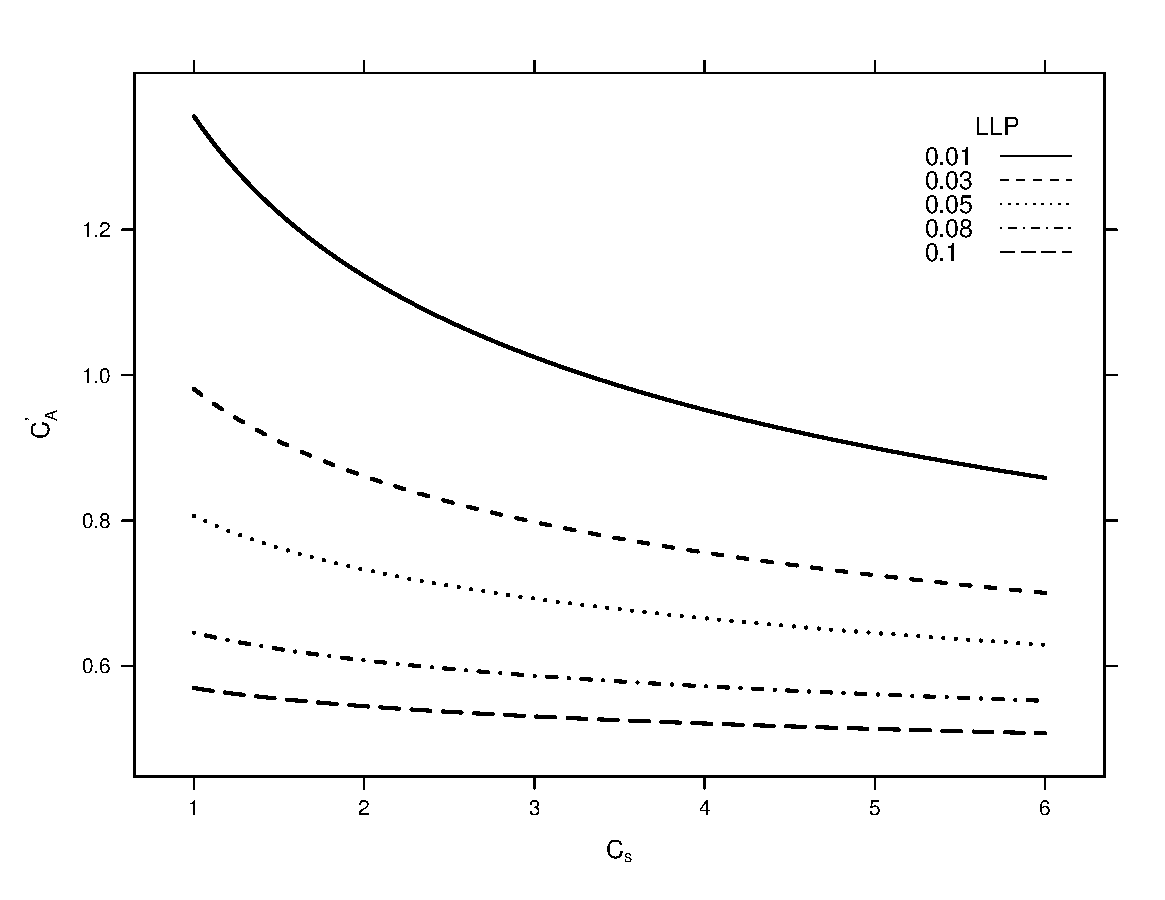
\includegraphics[width=.9\linewidth]{../figs/CurvasLLP.pdf}
\end{frame}

\begin{frame}[label=sec-1-4-4]{Relación entre $C_{A}^{'}$ y LLP}
\begin{itemize}
\item $C_{s}=3$
\end{itemize}

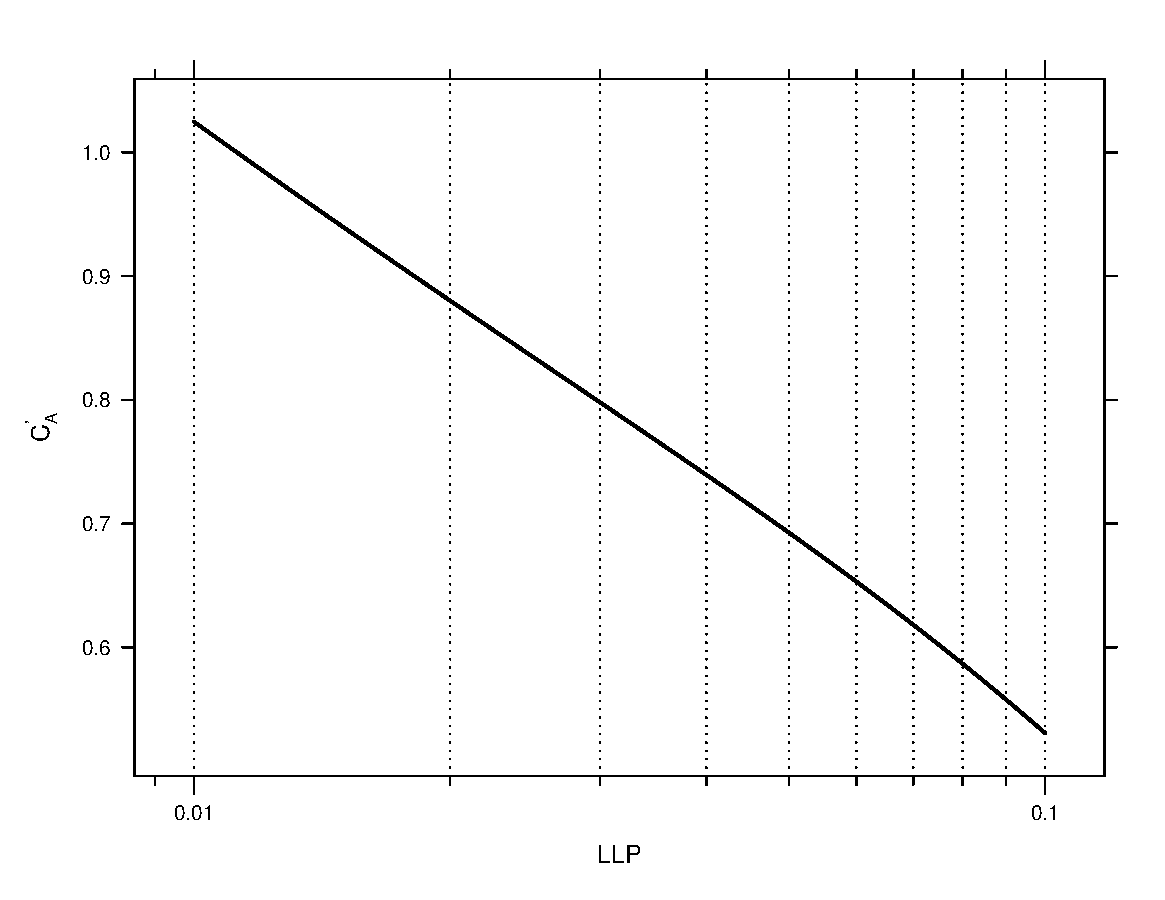
\includegraphics[width=.9\linewidth]{../figs/CurvasLLP_Cs3.pdf}
\end{frame}

\begin{frame}[label=sec-1-4-5]{Método del LLP}
\begin{itemize}
\item Es posible ajustar las curvas isofiables a una ecuación analítica:
\end{itemize}

\[
C_{A}^{'} = f\cdot C_{s}^{-u}
\]

\begin{itemize}
\item $f$ y $u$ son dos parámetros sin significado físico, dependientes del lugar y del LLP deseado.
\item Para su determinación es necesario realizar varias simulaciones previas.
\end{itemize}
\end{frame}

\begin{frame}[label=sec-1-4-6]{Método de LLP}
\begin{itemize}
\item Este proceso de cálculo se apoya en series de valores de radiación solar que reproducen el comportamiento estadístico de la irradiación.

\item Predicción del comportamiento del sistema limitada por la incertidumbre asociada.

\item Los ejercicios de cálculo para probabilidades de pérdida de carga inferiores a $LLP=\num{1e-2}$ carecen de utilidad.
\end{itemize}

\begin{block}{Recordatorio}
\guillemotleft{}[\ldots{}] los modelos de simulación muy exactos pueden proporcionar números también muy exactos, pero ello no significa que se traduzcan automáticamente en predicciones también muy exactas.\guillemotright{}
\end{block}
\end{frame}

\begin{frame}[label=sec-1-4-7]{Método del mes peor}
\begin{block}{Valores según el UTS for SHS}
\begin{itemize}
\item Electrificación rural:

\begin{itemize}
\item $C_{A}=1.1$

\item $3\leq C_{S}\leq5$
\end{itemize}

\item Aplicaciones profesionales:

\begin{itemize}
\item $1.2\leq C_{A}\leq1.3$

\item $5\leq C_{S}\leq8$
\end{itemize}
\end{itemize}
\end{block}
\end{frame}

\subsection{Configuración de generador y batería}
\label{sec-1-5}
\begin{frame}[label=sec-1-5-1]{Configuración de generador y batería}
\begin{itemize}
\item Una vez elegidos los valores de $C_{A}$ y $C_{S}$, se deben configurar el generador y batería de acuerdo a las tensiones de trabajo.

\item En general, la batería impone la tensión de trabajo (no hay buscador de MPP). Supondremos $V_{mpp}\simeq V_{b}$

\item Carga en Ah
\end{itemize}
\[
Q_L = L / V_b
\]
\end{frame}

\begin{frame}[label=sec-1-5-2]{Batería}
\begin{itemize}
\item Capacidad en Ah (es recomendable no usar baterías en paralelo)
\end{itemize}
\[
Q_B = \frac{C_S \cdot Q_L}{PD}
\]

\begin{itemize}
\item Hay que elegir el número de vasos en serie adecuados a $V_b$
\end{itemize}
\end{frame}


\begin{frame}[label=sec-1-5-3]{Generador}
\begin{itemize}
\item Capacidad del generador
\end{itemize}
\begin{align*}
C_{A} &= \frac{\eta_{G}\cdot A_{G}\cdot\overline{G_{d}}(\beta,\alpha)}{Q_L \cdot V_b}\\
I_{g}^{*}\cdot V_{b} &= \eta_{G}\cdot A_{G}\cdot G_{stc} 
\end{align*}

\begin{itemize}
\item Corriente de funcionamiento (determina número de ramas)
\end{itemize}
\[
I_{g}^{*} &=  \frac{C_{A}\cdot Q_{L}\cdot G_{stc}}{\overline{G_{d}}(\beta,\alpha)}
\]

\begin{itemize}
\item Hay que elegir el número de módulos en serie adecuados a $V_b$
\end{itemize}
\end{frame}

\begin{frame}[label=sec-1-5-4]{Inclinación del generador}
\begin{itemize}
\item Para instalaciones con \alert{consumos constantes o similares a lo largo del año}, se busca maximizar la radiación en los meses de menor insolación $$\beta=|\phi|+10^{\circ}$$

\item Para instalaciones con \alert{consumo menor en meses de baja radiación} se busca maximizar radiación en equinoccios.$$\beta=|\phi|$$

\item Para instalaciones con \alert{uso predominante en verano} (hemisferio Norte) conviene emplear un ángulo inferior a la latitud. $$\beta=|\phi|-10^{\circ}$$

\item En general, la inclinación \alert{debe superar} los $15^{\circ}$.
\end{itemize}
\end{frame}

\section{Consumo}
\label{sec-2}

\subsection{Estimación del consumo}
\label{sec-2-1}
\begin{frame}[label=sec-2-1-1]{Cálculo del consumo}
$$L_{T}=\frac{L_{dc}}{\eta_{r}}+\frac{L_{ac}}{\eta_{inv}}$$

$$L=\frac{L_{T}}{\eta_{bat}\cdot\eta_{c}}$$

Como valores orientativos pueden utilizarse

$\eta_{inv}=0.9$, $\eta_{r}=0.95$, $\eta_{bat}=0.85$ y $\eta_{c}=0.98$.
\end{frame}

\begin{frame}[label=sec-2-1-2]{Distribución del consumo}
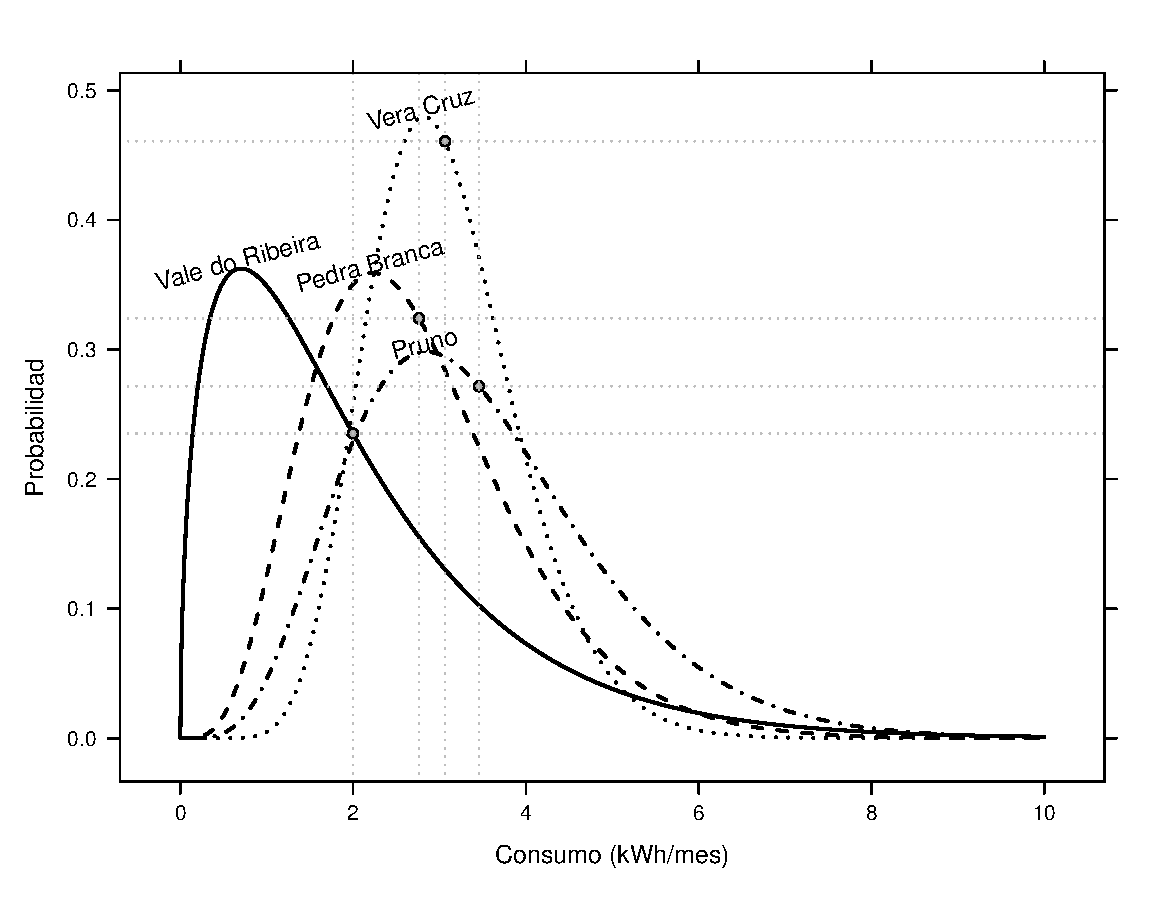
\includegraphics[width=.9\linewidth]{../figs/ConsumoGamma.pdf}
\end{frame}

\begin{frame}[label=sec-2-1-3]{Relación entre el consumo y la fiabilidad}
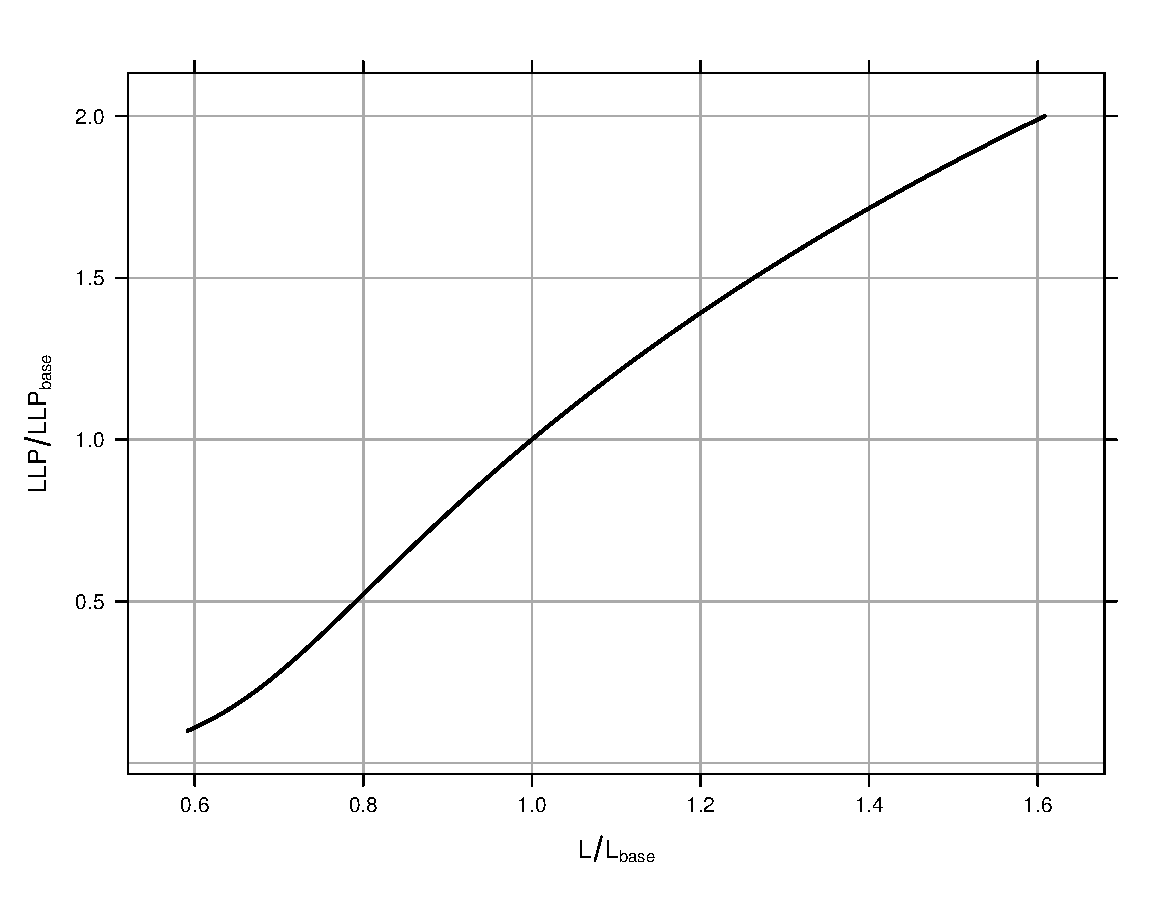
\includegraphics[width=.9\linewidth]{../figs/ConsumoLLP.pdf}
\end{frame}

\subsection{Escenarios}
\label{sec-2-2}
\begin{frame}[label=sec-2-2-1]{SHS 1}
\begin{block}{120 Wh/dia}
\begin{itemize}
\item Iluminación

\item Radio

\item TV b/n,

\item Sin frigorífico
\end{itemize}
\end{block}

\begin{block}{Valores recomendados}
$$\begin{aligned}
C_{A} & = & 1.1\\
3\leq & C_{s} & \leq5
\end{aligned}$$
\end{block}
\end{frame}

\begin{frame}[label=sec-2-2-2]{SHS 2}
\begin{block}{250 Wh/dia}
\begin{itemize}
\item Iluminación

\item Radio

\item TV color

\item Sin frigorífico
\end{itemize}
\end{block}

\begin{block}{Valores recomendados}
$$\begin{aligned}
C_{A} & = & 1.1\\
3\leq & C_{s} & \leq5
\end{aligned}$$
\end{block}
\end{frame}

\begin{frame}[label=sec-2-2-3]{SHS 3}
\begin{block}{1000 Wh/dia}
\begin{itemize}
\item Iluminación

\item radio

\item TV color

\item Con frigorífico eficiente
\end{itemize}
\end{block}

\begin{block}{Valores recomendados}
$$\begin{aligned}
C_{A} & = & 1.1\\
C_{S} & = & 5
\end{aligned}$$
\end{block}
\end{frame}

\begin{frame}[label=sec-2-2-4]{Centrales}
\begin{block}{}
\begin{itemize}
\item Todo AC

\item 500 Wh/dia por vivienda.
\end{itemize}
\end{block}

\begin{block}{Valores recomendados}
$$\begin{aligned}
C_{A} & = & 1.1\\
C_{S} & = & 5\end{aligned}$$
\end{block}
\end{frame}
% Emacs 24.4.1 (Org mode 8.2.7c)
\end{document}